
% This is misnamed filename. We wanted this to be the inrtoduction to
% the idea of adaptive runtime system

%\begin{frame}[fragile]
%\frametitle{An Empowered Runtime System}

%\begin{itemize}
%\item Think now, based on the model so far, what the runtime system
%  can do
%\item It is free to migrate chares across processors, as and when it pleases
%\item It is free to schedule the method invocations (including
%  constructors) that are waiting in the Queue on a processor in any
%  order it pelases
%\item Automatic Instrumentation
%\begin{itemize}
%\item It schedules invocations: so it knows how long they take
%\item It mediates communication: so it knows which chares talk to whom
%\end{itemize}
%
%\end{itemize}
%
%\end{frame}
%
%\begin{frame}[fragile]
%\frametitle{An Introspecitve and Adaptive Runtime System (CHANGE FIG)}
%\begin{itemize}
%\item Based on these capabilities, Charm++ runtime includes:
%\begin{itemize}
%\item Load balancing Schemes
%\item Fault Tolerance Schemes
%\item Communication optimizers
%\end{itemize}
%\end{itemize}
%
%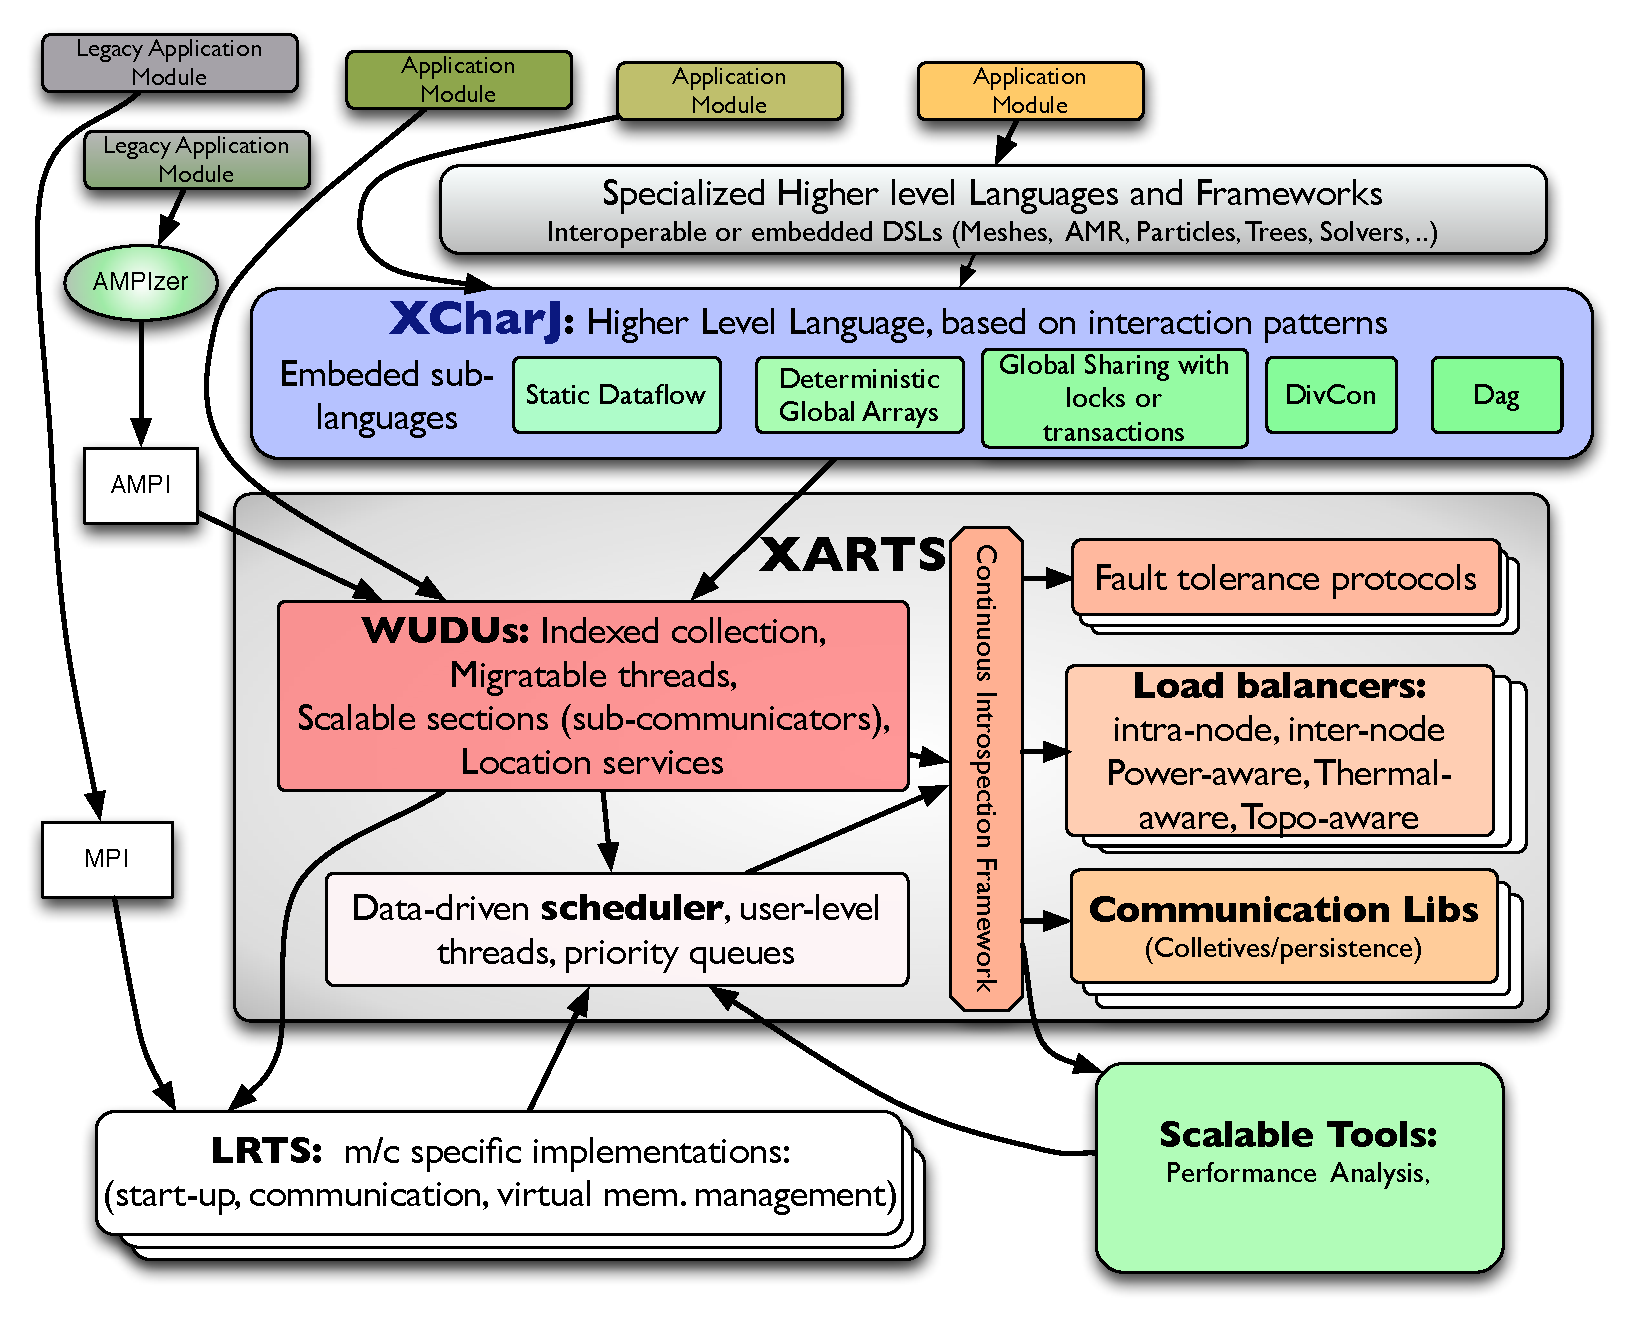
\includegraphics[width=0.8\textwidth]{figures/arts}
%
%\end{frame}

\begin{frame}[fragile]
\frametitle{Chare Migration: motivations}
\begin{itemize}
\item Chares are initially placed according to a placement map
\begin{itemize}
\item The user can specify this map
\end{itemize}
\item While running, some processors might be overloaded
\begin{itemize}
\item Need to rebalance the load
\end{itemize}
\item Automatic checkpoint
\begin{itemize}
\item Migration to disk
\end{itemize}
\item Chares are made serializable for transport using the Pack UnPack (PUP) framework
\end{itemize}
\end{frame}

\begin{frame}[fragile]
\frametitle{The PUP Process}
  \begin{center}
    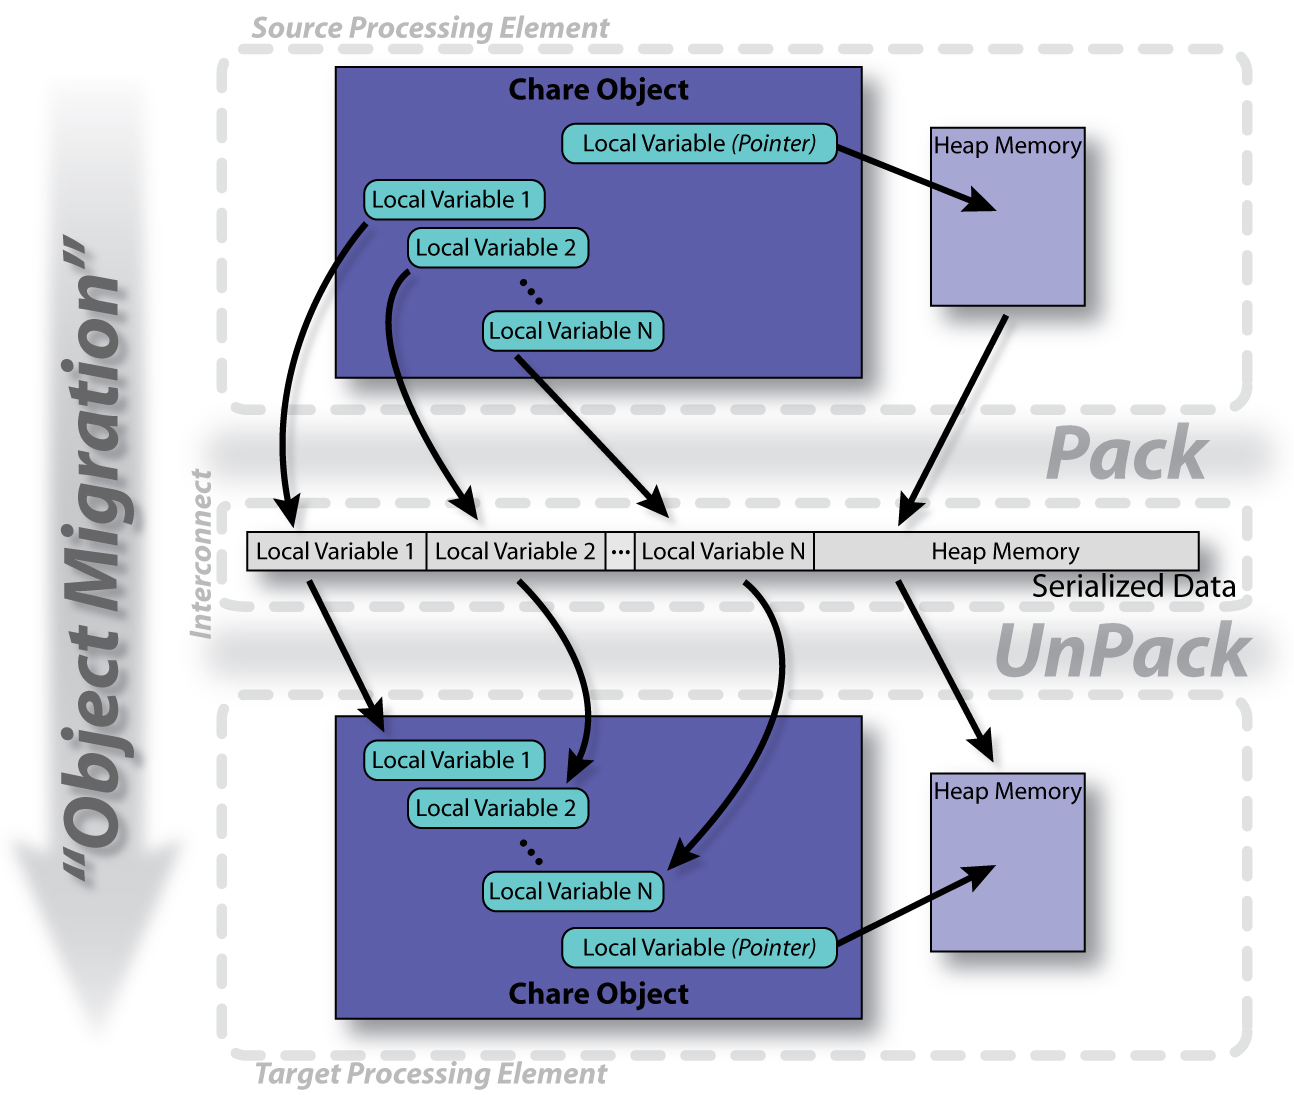
\includegraphics[width=0.8\textwidth]{figures/PUPProcess.png}
  \end{center}
\end{frame}

\comment{
\begin{frame}[fragile]
\frametitle{PUP Usage Sequence}
  \begin{center}
    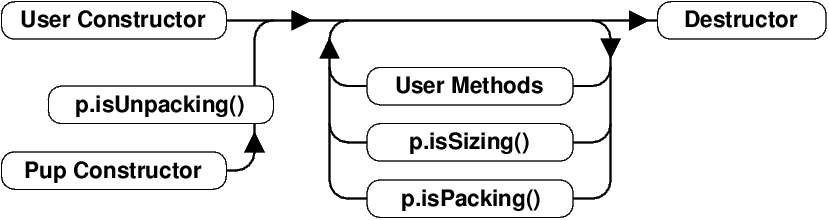
\includegraphics[width=0.8\textwidth]{figures/PUPUsage.png}
  \end{center}
\begin{columns}
 \begin{column}{0.5\textwidth}
 \begin{itemize}
 \item Migration out:
 \begin{itemize}
 \item ckAboutToMigrate
 \item Sizing
 \item Packing
 \item Destructor
 \end{itemize}
 \end{itemize}
 \end{column}
 \begin{column}{0.5\textwidth}
 \begin{itemize}
 \item Migration in:
 \begin{itemize}
 \item Migration constructor
 \item UnPacking
 \item ckJustMigrated
 \end{itemize}
 \end{itemize}
\end{column}
\end{columns}
\end{frame}
}

\begin{frame}[fragile]
\frametitle{Writing a PUP routine}
 \begin{columns}
 \begin{column}{0.5\textwidth}
   \begin{lstlisting}
class MyChare : public CBase_MyChare {
  int a;   float b;   char c;
  float localArray[LOCAL_SIZE];
  int heapArraySize;
  float* heapArray;
  MyClass *pointer;
 
  public:
   MyChare();
   MyChare(CkMigrateMessage *msg) {};
   ~MyChare() {
     if (heapArray != NULL) {
       delete [] heapArray;
       heapArray = NULL;
     }
};
 \end{lstlisting}
 \end{column}
 \begin{column}{0.5\textwidth}
  \begin{lstlisting}
void pup(PUP::er &p) {
   CBase_MyChare::pup(p);
   p | a;  p | b; p | c;
   p(localArray, LOCAL_SIZE);
   p | heapArraySize;
   if (p.isUnpacking()) {
     heapArray = new float[heapArraySize];
   }
   p(heapArray, heapArraySize);
   int isNull = (pointer==NULL) ? 1 : 0;
   p | isNull;
   if (!isNull) {
     if (p.isUnpacking()) pointer = new MyClass();
     p | *pointer;
   }
 }
}
  \end{lstlisting}
  \end{column}
  \end{columns}
\end{frame}

\comment{
\begin{frame}[fragile]
\frametitle{PUP: Concerns}
\begin{itemize}
\item If variables are added to an object, update the PUP routine
\item If the object allocates data on the heap, copy it recursively, not just the pointer
\item Remember to allocate memory while unpacking
\item Sizing, Packing, and Unpacking must scan the same variables in the same order
\item Test PUP routines with “+balancer RotateLB”
\end{itemize}
\end{frame}
}
\transition{Controlling Placement}

\begin{frame}[fragile]
  \frametitle{Static Mapping}
  \framesubtitle{Motivation}
  \begin{itemize}
    \item In some applications, load patterns don’t change much as computation progresses
    \begin{itemize}
      \item You, the programmer, may want to control which chare lives on which processors
      \item This is also true when  load may evolve over time, but you want to control initial placement of chares
    \end{itemize}
    \item The feature in Charm++ for this purpose is called Map Objects
    \begin{itemize}
      \item Sec. 13.2.2 of the Charm++ manual
    \end{itemize}
  \end{itemize}
\end{frame}

\begin{frame}[fragile]
  \frametitle{Static Mapping}
  \framesubtitle{CkArrayOption Syntax}
  \begin{itemize}
    \item To specify static initial mapping, we must first learn this feature
    \begin{itemize}
      \item Whenever a chare array is created, one can pass an optional parameter of type CkArrayOptions
    \end{itemize}
    \item \code{CkArrayOptions opts(numElements);}
    \item Set properties in opts (e.g. opts.setAnytimeMigration(false); )
    \item \code{P = Cproxy\_A::CkNew(parameters, opts);}
    \item Many propperties of arrays can be set using this method.
    \item In particular, we can specify a map object
  \end{itemize}
\end{frame}

\begin{frame}[fragile]
  \frametitle{Static Mapping}
  \framesubtitle{CkArrayMap Syntax}
  \begin{lstlisting}
class CkArrayMap : public Group {
  public:
  // ...
  // Return an ``arrayHdl'', given some information about the array
  virtual int registerArray(CkArrayIndex& numElements,CkArrayID aid);
  // Return the home processor number for this element of this array
  virtual int procNum(int arrayHdl,const CkArrayIndex &element);
};
  \end{lstlisting}
  \begin{itemize}
    \item If you want to specify a map for a chare array you are about to create, you must first define a subclass of CkArrayMap
    \item It is a “Group”.. More on that much later
    \begin{itemize}
      \item You don’t need to know any more than inheriting from it for now
    \end{itemize}
  \end{itemize}
\end{frame}

\begin{frame}[fragile]
  \frametitle{Static Mapping}
  \framesubtitle{Customized CkArrayMap Syntax}
  \begin{lstlisting}
class BlockMap : public CkArrayMap {
public:
  BlockMap(void) {}
  BlockMap(CkMigrateMessage *m){}
  int registerArray(CkArrayIndex& numElements,CkArrayID aid) { return 0;}
  int procNum(int /*arrayHdl*/,const CkArrayIndex &idx) {
    int elem=*(int *)idx.data();
    int penum =  (elem/(32/CkNumPes()));
    return penum;
  }
};
    \end{lstlisting}
  \begin{itemize}
    \item CkArrayIdx is a datatye that’s normally used by the system. You can peek into it to extract indices. The example works for 1D array
  \end{itemize}
\end{frame}

\begin{frame}[fragile]
  \frametitle{Static Mapping}
  \framesubtitle{Using A Custom Map}
  \begin{lstlisting}
  // Create the map group
  CProxy_BlockMap myMap = CProxy_BlockMap::ckNew();
  // Make a new array using that map
  CkArrayOptions opts(nElements);
  opts.setMap(myMap);
  a1 = CProxy_A1::ckNew( parameters,opts);
  \end{lstlisting}
  \begin{itemize}
    \item Create a map object, 
    \item pass it to an CkArrayOptions object (opts here), and then 
    \item pass that to ckNew
  \end{itemize}
\end{frame}
